% !TeX document-id = {66b2d4b6-7613-4c19-b40c-a50fc00d38ff}
% !TeX program = lualatex
% !BIB program = biber
% Lualatex is important to render TTF fonts; with pdflatex it's just the regular one
% ratio 16:9 -- https://tex.stackexchange.com/questions/14336/

% compile two versions, inspired by https://tex.stackexchange.com/a/1501
% use the script "compile-pdf.sh"
\newif\ifhandout
% if flags.tex does not exist, create an empty file to be able to compile in TeXstudio
\input{flags}

\ifhandout
\documentclass[12pt,aspectratio=169,handout]{beamer}
\else
\documentclass[12pt,aspectratio=169]{beamer}
\fi

% adjust for 16:9
% https://tex.stackexchange.com/questions/354022/modifying-the-margins-of-all-slides-in-beamer
\setbeamersize{text margin left=0.3cm,text margin right=4.5cm} 

%\usepackage{xcolor}

% use Metropolis as the basis theme
\usetheme[subsectionpage=progressbar]{metropolis}
% blocks with background globally
\metroset{block=fill}

% ------- Paderborn specifics ----------
\usepackage{fontspec}
%\setsansfont{karla} % looked bad, too fat
\setsansfont{Segoe UI} % looks OK-ish

% Paderborn color scheme
\definecolor{UPBUltraBlue}{RGB}{0, 37, 170}

\setbeamercolor{frametitle}{bg=white, fg=UPBUltraBlue}

% name in footer
\setbeamertemplate{frame numbering}{Prof.\ Dr.\ Ivan Habernal ~ | ~ \insertframenumber }

% adjust the background to be completely white
\setbeamercolor{background canvas}{bg=white}

% add Paderborn logo at each slide
% actually not -- it's just eating up space
%\addtobeamertemplate{frametitle}{}{%
	%\begin{tikzpicture}[remember picture,overlay]
	%	\node[anchor=north east,yshift=2pt] at (current page.north east) {\includegraphics[height=0.9cm]{img/UPB_Logo_ENG_coloured_RGB}};
	%\end{tikzpicture}
	%}

% show TOC at every section start
\AtBeginSection{
	\frame{
		\vspace{2em}
		\sectionpage
		\hspace*{2.2em}\begin{minipage}{10cm}
			\tableofcontents[currentsection]
		\end{minipage}
		% we need the logo to show up here as well
		\begin{tikzpicture}[remember picture,overlay]
			\node[anchor=north east,yshift=2pt] at (current page.north east) {\includegraphics[height=0.9cm]{img/UPB_Logo_ENG_coloured_RGB}};
		\end{tikzpicture}
	}
}
% ------- end of Paderborn specifics ----------


% typeset mathematics on serif
\usefonttheme[onlymath]{serif}

% better bibliography using biber as backend
\usepackage[natbib=true,backend=biber,style=authoryear-icomp,maxbibnames=30,maxcitenames=9,uniquelist=false,giveninits=true,doi=false,url=false,dashed=false,isbn=false]{biblatex}
% shared bibliography
\addbibresource{../nlpwdl-bibliography.bib}
% disable "ibid" for repeated citations
\boolfalse{citetracker}



\usepackage{xspace}


% for derivatives, https://tex.stackexchange.com/a/412442
\usepackage{physics}

\usepackage{tikz}
\usetikzlibrary{matrix, positioning}
\usetikzlibrary{angles,quotes} % for angles
\usetikzlibrary{backgrounds} % background
\usetikzlibrary{decorations.pathreplacing} % curly braces
\usetikzlibrary{calligraphy}
\usetikzlibrary{calc} % for neural nets

% for plotting functions
\usepackage{pgfplots}
\usepgfplotslibrary{dateplot}

% sub-figures
\usepackage{caption}
\usepackage{subcaption}

% book tabs
\usepackage{booktabs}


% argmin, argmax
\usepackage{amsmath}
\DeclareMathOperator*{\argmax}{arg\!\max}
\DeclareMathOperator*{\argmin}{arg\!\min}
% softmax
\DeclareMathOperator*{\softmax}{soft\!\max}

% bold math
\usepackage{bm}

% for \mathclap
\usepackage{mathtools}

% algorithms
\usepackage[noend]{algpseudocode}


% for neurons and layers in tikz
\tikzset{
	neuron/.style={draw, rectangle, inner sep=2pt, minimum width=0.75cm, fill=blue!20},
	param/.style={draw, rectangle, inner sep=2pt, minimum width=0.75cm, fill=green!20},
	constant/.style={draw, rectangle, inner sep=2pt, minimum width=0.75cm, fill=black!15},
	% for citation nodes right top
	ref/.style={anchor = north east, text width=7.8cm, yshift=-1.3cm, xshift=-0.2cm, scale=0.5},
	state/.style={rectangle, inner sep=2pt, minimum width=0.75cm, fill=black!5},
}

% for strike-through text (added in Lecture 06)
\usepackage[normalem]{ulem}

% added in Lecture 7
% RNN
\DeclareMathOperator*{\rnn}{RNN}
% RNN star
\DeclareMathOperator*{\rnnstar}{RNN^{*}}
% bi-RNN
\DeclareMathOperator*{\birnn}{biRNN}


% added in Lecture 9
\usetikzlibrary{fit} % for hightligting by calling "fit"

% algorithms
\usepackage[noend]{algpseudocode}


\title{Natural Language Processing with Deep Learning}
\subtitle{Lecture 10 -- Text classification 6: BERT part two}
\date{December 15, 2023}
\author{Prof.\ Dr.\ Ivan Habernal}
\institute{Natural Language Processing Group 
	\hfill \includegraphics[height=1.4cm]{img/UPB_Logo_ENG_coloured_RGB} \\
	Paderborn University \\
	We focus on Trustworthy Human Language Technologies \hfill \texttt{www.trusthlt.org} }

\begin{document}

\maketitle

\iffalse
\section{BERT (finishing)}


\subsection{Input and pre-training}

\begin{frame}{BERT: Tokenization}
	
	Tokenizing into a multilingual WordPiece inventory
	
	\begin{itemize}
		\item Recall that WordPiece units are sub-word units
		\item 30,000 WordPiece units (newer models 110k units, 100 languages)
	\end{itemize}
	
	Implications: BERT can "consume" any language
	
	
\end{frame}


\begin{frame}{BERT: Input representation}
	
	\begin{itemize}
		\item Each WordPiece token from the input is represented by a \textbf{WordPiece embedding} (randomly initialized)
		\item Each position from the input is associated with a \textbf{positional embedding} (also randomly initialized)
		\item Input length limited to \textbf{512} WordPiece tokens, using \texttt{<PAD>}ding
		\item Special tokens
		\begin{itemize}
			\item The fist token is always a special token \textbf{[CLS]}
			\item If the task involves two sentences (e.g., NLI), these two sentences are separated by a special token \textbf{[SEP]}; also special two \textbf{segment position embeddings} 
		\end{itemize}
		
	\end{itemize}
	
\end{frame}


\begin{frame}{BERT: Input representation summary}
	
	\begin{figure}
		\includegraphics[width=\linewidth]{img/bert-input.png}	
	\end{figure}
	
\end{frame}


\subsection{Pre-training}


\begin{frame}{BERT: Self-supervised multi-task pre-training}
	
	Prepare two auxiliary tasks that need no labeled data
	
	\bigskip
	
	\begin{columns}
		\begin{column}{0.5\linewidth}
			\begin{small}
				Task 1: Cloze-test task
				\begin{itemize}
					\item 	Predict the masked WordPiece unit (multi-class, 30k classes)
				\end{itemize}
				
				
				Task 2: Consecutive segment prediction
				
				\begin{itemize}
					\item Did the second text segment appeared after the first segment? (binary)
				\end{itemize}
			\end{small}
			
		\end{column}
		\begin{column}{0.5\linewidth}
			
			\begin{figure}
				\includegraphics[width=\linewidth]{img/bert-pretraining.png}
			\end{figure}
		\end{column}
		
	\end{columns}
\end{frame}




\begin{frame}{BERT: Pre-training data generation}
	
	Take the entire Wikipedia (in 100 languages; 2,5 billion words)
	
	To generate a single training instance, sample two segments (max combined length 512 WordPiece tokens)
	
	\begin{itemize}
		\item For Task 2, replace the second segment randomly in 50\% (negative samples)
		\item For Task 1, choose random 15\% of the tokens, and in 80\% replace with a [MASK] 
	\end{itemize}
	
	
\end{frame}


\begin{frame}{BERT: Pre-training data -- Simplified example}
	
	\begin{columns}
		\begin{column}{0.5\linewidth}
			\begin{figure}
				\includegraphics[width=\linewidth]{img/bert-pretraining2.png}
			\end{figure}
		\end{column}
		\begin{column}{0.5\linewidth}
			\begin{small}
				
				\begin{itemize}
					\item $<$PAD$>$ding is missing
					\item The actual segments are longer and not necessarily actual sentences (just spans)
					\item The WordPiece tokens match full words / morphology well in this English text, but recall the ones we have seen before
				\end{itemize}
			\end{small}
		\end{column}
	\end{columns}
	
	
\end{frame}



\subsection{Downstream tasks and fine-tuning}

\begin{frame}{BERT: Representing various NLP tasks}
	
	\begin{figure}
		\includegraphics[width=0.5\linewidth]{img/task1.png}
	\end{figure}
	
	That explains the special [CLS] token at sequence start
	
\end{frame}



\begin{frame}{BERT: Representing various NLP tasks}
	
	\begin{figure}
		\includegraphics[width=0.6\linewidth]{img/task2.png}
	\end{figure}
	
	
\end{frame}



\begin{frame}{BERT: Representing various NLP tasks}
	
	\begin{figure}
		\includegraphics[width=0.5\linewidth]{img/task3.png}
	\end{figure}
	
	
	Not conditioned on surrounding predictions	
	
\end{frame}

\begin{frame}{BERT: Very abstract view}
	
	\begin{figure}
		\includegraphics[width=\linewidth]{img/bert1.png}
	\end{figure}	
	
\end{frame}


\begin{frame}{BERT: Very abstract view}
	
	\begin{figure}
		\includegraphics[width=\linewidth]{img/bert1.png}
	\end{figure}	
	
	Pretraining BERT took originally 4 days on 64 TPUs\footnote{Can be done more efficiently, see, e.g., \citet{izsak-etal-2021-train}}
	
	\bigskip
	
	Once pre-trained, transfer and "fine-tune" on your small-data task and get competitive results


	
\begin{tikzpicture}[overlay, remember picture] 
	\node at (current page.north east)[ref] {\fullcite{izsak-etal-2021-train} \par};
\end{tikzpicture}

	
\end{frame}


\begin{frame}{Recap}
	
	BERT stays on the shoulders of many clever concepts and techniques, mastered into a single model
	
\textbf{What do we know about how BERT works?}

	
\emph{``BERTology has clearly come a long way, but it is fair to say we still have more questions than answers about how BERT works.''} --- \citet{Rogers.et.al.2020.BERT}\footnote{Highly recommended reading!}
	
	
\begin{tikzpicture}[overlay, remember picture] 
	\node at (current page.north east)[ref] {\fullcite{Rogers.et.al.2020.BERT} \par};
\end{tikzpicture}
	
\end{frame}


\fi

\begin{frame}{Multi-head bidirectional / unmasked self-attention}
	
\begin{minipage}[t][10cm][t]{15cm}

Input: $\bm{X} \in \mathbb{R}^{\ell_{\text{x}} \times d_{\text{x}}}$, vector representations of the sequence of length $\ell_{\text{x}}$

Output: $\bm{\tilde{V}} \in \mathbb{R}^{\ell_{\text{x}} \times d_{\text{out}}}$, updated vector representations of tokens in $\bm{X}$

Hyper-param: \colorbox{yellow!30}{$H$}, number of attention heads

Params for each {\colorbox{yellow!30}{$h \in [H]$}}: $\bm{\mathcal{W}_{qkv}}^h$:
\begin{itemize}
\item $\bm{W_q}^h, \bm{W_k}^h \in \mathbb{R}^{d_\text{x} \times d_\text{attn}}$,
$\bm{b_q}^h, \bm{b_k}^h \in \mathbb{R}^{d_\text{attn}}$,
$\bm{W_v} \in \mathbb{R}^{d_\text{x} \times d_\text{mid}}$, $ \bm{b_v} \in \mathbb{R}^{d_\text{mid}}$
\item {\colorbox{yellow!30}{$\bm{W_o}$}} $\in \mathbb{R}^{H \cdot d_\text{mid} \times d_\text{out}}$, {\colorbox{yellow!30}{$\bm{b_o}$}} $\in \mathbb{R}^{d_\text{out}}$	
\end{itemize}


\begin{algorithmic}[1]
\Function{MHAttention}{$\bm{X} ; \bm{\mathcal{W}}$}
\For{$h \in [H]$}
\State $\bm{Y}^h \gets \textsc{Attention}(\bm{X}; \bm{\mathcal{W}_{qkv}}^h)$
\Comment{$\bm{Y}^h \in \mathbb{R}^{\ell_{\text{x}} \times d_{\text{mid}}}}$
\EndFor
\State{$\bm{Y} \gets [\bm{Y}^1; \bm{Y}^2; \ldots; \bm{Y}^H]$}
\Comment{$\bm{Y} \in \mathbb{R}^{\ell_{\text{x}} \times H \cdot d_{\text{mid}}}}$
%\State $\bm{Q} \gets \bm{X} \bm{W_q} +_{\text{(rows)}} \bm{b_q}$
%\State $\bm{S} \gets \frac{1}{\sqrt{d_{\text{attn}}}} (\bm{Q} \bm{K}^\top)$
%\Comment{Scaled score $\in \mathbb{R}^{\ell_{\text{x}} \times \ell_{\text{x}}}$}
\State \Return $\bm{\tilde V} = \bm{Y} \bm{W_o} + \bm{b_o}$

\EndFunction
\end{algorithmic}

\end{minipage}
\end{frame}


\begin{frame}{GELU --- Gaussian Error Linear Units}
	
\begin{block}{Recall: CDF $\Phi(x)$ of standard normal $X \sim \mathcal{N}(0; 1)$}
$\Phi(x) = \Pr(X \leq x) = \frac{1}{\sqrt{2 \pi}} \int_{-\infty}^{x} \exp \left(
\frac{-t^2}{2} \right) \mathrm{d}t$
\end{block}
$$
\begin{aligned}
\textsc{GELU}(x) &= x \cdot \Phi(x) \\
&\approx x \cdot \sigma(1.702 x) \qquad \text{(if speed $>$ exactness)}
\end{aligned}
$$

\begin{figure}
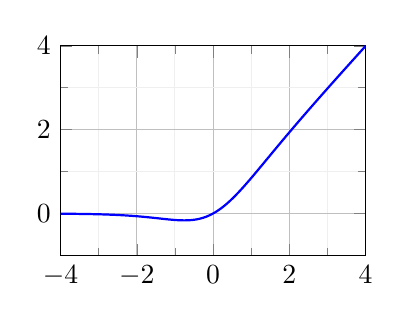
\begin{tikzpicture}

\begin{axis}[
	xmin = -4, xmax = 4,
	ymin = -1, ymax = 4,
	xtick distance = 2,
	ytick distance = 2,
	grid = both,
	minor tick num = 1,
	major grid style = {lightgray},
	minor grid style = {lightgray!25},
	width = 0.45\textwidth,
	height = 0.35\textwidth,
	legend pos = north west
	]
	
	\addplot[
	domain = -10:10,
	samples = 200,
	smooth,
	thick,
	blue,
	] {
		x * 1/(1 + exp(-1 * 1.702 * x))
	};
	
\end{axis}
\end{tikzpicture}
\end{figure}


	

\begin{tikzpicture}[overlay, remember picture] 
	\node at (current page.north east)[ref] {\fullcite{Hendrycks.Gimpel.2016.arXiv} \newline \newline
		For vectors $\bm{x} \in \mathbb{R}^n$, $\textsc{GELU}(\bm{x})$ is applied element-wise
		\par};
\end{tikzpicture}

	
\end{frame}


\begin{frame}{Simplifying notation: Perform \textsc{LayerNorm} on each row}
	
	\begin{block}{Recall: LayerNorm}
		Input: $\bm{e} \in \mathbb{R}^{d}$ (output of a layer), Output: $\bm{\hat e} \in \mathbb{R}^{d}$ \\
		Parameters: $\bm{\gamma}, \bm{\beta} \in \mathbb{R}^{d}$, element-wise scale and offset
		
		\begin{algorithmic}[1]
			\Function{LayerNorm}{$\bm{e} | \bm{\gamma}, \bm{\beta}$}
			\State $m \gets \frac{1}{d} \sum_{i = 1}^{d} \bm{e}[i]$
			\Comment{`Sample mean' of $\bm{e}$}
			\State $v \gets \frac{1}{d} \sum_{i = 1}^{d} (\bm{e}[i] - m)^2$
			\Comment{`Sample variance' of $\bm{e}$}
			\State \Return $\bm{\hat e} = \frac{\bm{e} - m}{\sqrt{v}} \odot \bm{\gamma} + \bm{\beta}$
			\Comment{Offset and scale}
			\EndFunction
		\end{algorithmic}
	\end{block}
	
	
	\begin{algorithmic}[1]
		\Function{LayerNormEachRow}{$\bm{X} \in \mathbb{R}^{m \times n} | \bm{\gamma}, \bm{\beta}$}
		\For{$t \in [m]$}
		\State $˝\bm{X}[t,:] \gets \textsc{LayerNorm}(\bm{X}{[t,:]} | \bm{\gamma}, \bm{\beta})$
		\EndFor
		\State \Return $\bm{X}$
		\EndFunction
	\end{algorithmic}
	
	
\end{frame}


\begin{frame}{BERT (Enc-Transformer) --- compute contextualized embeddings}

\begin{minipage}[t][10cm][t]{15cm}

Input: $\bm{x} \in V^*$, a sequence of token IDs

Output: $\bm{P} \in (0,1)^{\ell_{\text{x}} \times N_{\text{V}}}$, where each row of $\bm{P}$ is a distribution over the vocabulary

Hyperparameters: $\ell_{\text{max}}, L, H, d_{\text{e}}, d_{\text{mlp}}, d_{\text{f}} \in \mathbb{N}$

Parameters: $\bm{\theta}$ includes all of the following parameters:

$\bm{W_e} \in \mathbb{R}^{N_\text{V} \times d_\text{e}}$, $\bm{W_p} \in \mathbb{R}^{\ell_{\text{max}} \times d_\text{e}}$, the token and positional embedding matrices

For $l \in [L]$:

$\bm{\mathcal{W}}_l$, multi-head attention parameters for layer $l$

$\bm{\gamma^1}_l, \bm{\beta^1}_l, \bm{\gamma^2}_l, \bm{\beta^2}_l$, two sets of layer-norm parameters

$\bm{W}^{\text{mlp1}}_l \in \mathbb{R}^{d_{\text{e}} \times d_\text{mlp}}$, $\bm{b}^{\text{mlp1}}_l \in \mathbb{R}^{d_\text{mlp}}$

$\bm{W}^{\text{mlp2}}_l \in \mathbb{R}^{d_\text{mlp} \times d_{\text{e}}}$, $\bm{b}^{\text{mlp2}}_l \in \mathbb{R}^{d_\text{e}}$


$\bm{W_f} \in \mathbb{R}^{d_\text{e} \times d_\text{f}}, \bm{b_f} \in \mathbb{R}^{d_\text{f}}$, $\bm{\gamma},\bm{\beta} \in \mathbb{R}^{d_\text{f}}$, the final linear projection and layer-norm parameters.


$\bm{W_u} \in \mathbb{R}^{d_\text{e} \times N_\text{V}}$, the unembedding matrix

\end{minipage}
\end{frame}





\begin{frame}{BERT (encoding-only transformer, forward pass)}

\vspace{-2em}
\begin{minipage}[t][10cm][t]{15cm}
\begin{algorithmic}[1]
\Function{ETransformer}{$\bm{x} ; \bm{\mathcal{W}}$}
\State $\ell \gets \text{length}(\bm{x})$
\State for $t \in [\ell]: \bm{e}_t \gets \bm{W_e}[x[t],:] + \bm{W_p}[t,:]$
\Comment{Token emb. + positional emb.}
\State $\bm{X} \gets \text{Stack row-wise}[\bm{e}_1, \bm{e}_2, \ldots \bm{e}_{\ell}]$
\For{$l = 1, 2, \dots, L$}
\State $\bm{X} \gets \bm{X} + \textsc{MHAttention}(\bm{X} | \bm{\mathcal{W}}_l)$
\Comment{Multi-head att., residual conn}
\State $\bm{X} \gets \textsc{LayerNormPerRow}(\bm{X} | \bm{\gamma^1}_l, \bm{\beta^1}_l)$
\State $\bm{X} \gets \bm{X} + \left(
\textsc{GELU}(\bm{X} \bm{W}^\text{mlp1}_l +_{\text{(row)}} \bm{b}^\text{mlp1}_l )
\bm{W}^{\text{mlp2}}_l +_{\text{(row)}} \bm{b}^{\text{mlp2}}_l \right)$
\Comment{MLP}
\State $\bm{X} \gets \textsc{LayerNormPerRow}(\bm{X} | \bm{\gamma^2}_l, \bm{\beta^2}_l)$
\EndFor
\State $\bm{X} \gets \textsc{GELU}(\bm{X} \bm{W_f}  +_{\text{(row)}} \bm{b_f} )$
\State $\bm{X} \gets \textsc{LayerNormPerRow}(\bm{X} | \bm{\gamma}_l, \bm{\beta}_l)$
\State \Return $\bm{P} = \softmax(\bm{X} \bm{W_u}) $
\Comment{Project to vocab., probabilities}
\EndFunction
\end{algorithmic}

\end{minipage}
\end{frame}



\begin{frame}{BERT (training by masked language modeling)}


%Output: $\bm{\hat{\theta}}$ trained parameters

%Hyperparameters: $p_{\text{mask}} \in (0, 1)$, $N_\text{epochs}$, $\eta$

\begin{minipage}[t][10cm][t]{15cm}
\begin{algorithmic}[1]
\Function{ETraining}{$\left\{ \bm{x}_n \right\}_{n = 1}^{N_\text{data}}$ sequences,  $\bm{\theta}$ init.\ params; $p_{\text{mask}} \in (0, 1)$, $N_\text{epochs}$, $\eta$}
\For{$i \in [N_{\text{epochs}}]$}
\For{$n \in [N_{\text{data}}]$}
	\State $\ell \gets \text{length}(\bm{x}_n)$
	\For{$t \in [\ell]$}
	\State $\tilde{\bm{x}}_n[t] \gets \texttt{<mask\_token>}$ with prob.\ $p_{\text{mask}}$, otherwise $\bm{x}_n[t]$
	\EndFor
	\State $\tilde{T} \gets \left\{ t \in [\ell] : \tilde{\bm{x}}_n[t] = \texttt{<mask\_token>} \right\}$
	\Comment{Indices of masked tokens}
	\State $\bm{P_{\theta}} \gets \textsc{ETransformer}(\tilde{\bm{x}}_n | \bm{\theta})$
	\State $\text{loss}_{\bm{\theta}} \gets - \sum_{t \in \tilde{T}} \log \bm{P_{\theta}} [t, \bm{x}_n[t]] $
	\State $\bm{\theta} \gets \bm{\theta} - \eta \cdot \nabla \text{loss}_{\bm{\theta}}$
\EndFor
\EndFor
\State \Return $\bm{\theta}$
\EndFunction
\end{algorithmic}

\end{minipage}
\end{frame}


\begin{frame}{Simple example explaining lines 6--7 (masking)}
$
\begin{pmatrix}
	\text{The} &
	\text{cat} &
	\text{sat}
\end{pmatrix}
\rightarrow
\bm{x}_n =
\begin{pmatrix}
	21 &
	11987 &
	5438
\end{pmatrix}
\quad \text{(Indices in $V$)}
$

Random masking (index of \texttt{<mask\_token>} = 50001):
\begin{enumerate}
\item For $t = 1$, the random outcome is "mask"
\item For $t = 2$, the random outcome is "keep"
\item For $t = 3$, the random outcome is "mask"
\end{enumerate}
$
\bm{\tilde{x}}_n =
\begin{pmatrix}
	50001 &
	11987 &
	50001
\end{pmatrix},
\tilde{T} = \left\{ 1, 3 \right\}
$

	
	
\end{frame}



\begin{frame}{Explaining line 9 (negative log likelihood)}
	
$
\begin{pmatrix}
	\text{The} &
	\text{cat} &
	\text{sat}
\end{pmatrix}
\rightarrow
\bm{x}_n =
\begin{pmatrix}
	21 &
	11987 &
	5438 
\end{pmatrix},
\bm{\tilde{x}}_n =
\begin{pmatrix}
	50001 &
	11987 &
	50001
\end{pmatrix},
\tilde{T} = \left\{ 1, 3 \right\}
$

$\bm{P_{\theta}} \gets \textsc{ETransformer}(\tilde{\bm{x}}_n | \bm{\theta})$
$$
\bm{P_{\theta}} =
\begin{pmatrix}
0.001 & 0.0007 & \ldots & 0.0003 \\
0.0013 & 0.0065 & \ldots & 0.0001 \\
0.079 & 0.015 & \ldots & 0.0001 \\
\end{pmatrix}
$$

$\bm{P_{\theta}} \in (0,1)^{\ell_{\text{x}} \times N_{\text{V}}}$, where each row of $\bm{P}$ is a distribution over the vocabulary

\end{frame}


\begin{frame}{Explaining line 9 (negative log likelihood)}

\begin{small}
$\bm{x}_n = (21, 11987, 5438), \bm{\tilde{x}}_n = (50001, 11987, 50001), \tilde{T} = \left\{ 1, 3 \right\}$

$
\bm{P_{\theta}} =
\begin{pmatrix}
	0.001 & \ldots & 0.0041_{21} & \ldots 0.0003 \\
	\vdots &  &  &  \\
\end{pmatrix}
$
\end{small}	

For $t = 1$, the model should learn to predict "The" (index 21)

Gold: $\bm{y} = (0, 0, \ldots, 1_{21}, \ldots, 0) \in \mathbb{R}^{N_{\text{V}}}$

Pred: $\bm{\hat{y}} = \bm{P_{\theta}}[1,:] = (0.001, \ldots, 0.0041_{21}, \ldots 0.0003) \in \mathbb{R}^{N_{\text{V}}}$

\begin{block}{Categorical cross entropy loss (Lec.\ 4)}
$L (\bm{\hat{y}, \bm{y}}) := - \sum_{k = 1}^{K} \bm{y}_{[k]} \log \left(  \bm{\hat{y}}_{[k]} \right)$ \\
$= - 1 \cdot \log (\bm{\hat{y}}[21])
= - \log(\bm{P_{\theta}}[1, 21])$ \\
$= - \log(\bm{P_{\theta}}[1, \bm{x}_n[1]]) 
= - \log(\bm{P_{\theta}}[t, \bm{x}_n[t]])$	
\end{block}

\end{frame}


\begin{frame}{Explaining line 9 (negative log likelihood)}
	
	\begin{small}
		$\bm{x}_n = (21, 11987, 5438), \bm{\tilde{x}}_n = (50001, 11987, 50001), \tilde{T} = \left\{ 1, 3 \right\}$
		
		$
		\bm{P_{\theta}} =
		\begin{pmatrix}
			\vdots &  \cdots &  \cdots &  \\
		\end{pmatrix}
		$
	\end{small}	
	
	For $t = 3$, the model should learn to predict "sat" (index 5438)
	
	\begin{block}{Categorical cross entropy loss}
		$L (\bm{\hat{y}, \bm{y}}) := - \sum_{k = 1}^{K} \bm{y}_{[k]} \log \left(  \bm{\hat{y}}_{[k]} \right)$ \\
		$= - 1 \cdot \log (\bm{\hat{y}}[5438])
		= - \log(\bm{P_{\theta}}[3, 5438])
		= - \log(\bm{P_{\theta}}[t, \bm{x}_n[t]])$	
	\end{block}
	

Sum over all masked token positions in $\tilde{T}$ gives us line 9:\\
$$\text{loss}_{\bm{\theta}} \gets - \sum_{t \in \tilde{T}} \log \bm{P_{\theta}} [t, \bm{x}_n[t]] $$
	
\end{frame}


\begin{frame}{License and credits}

	\begin{columns}
		\begin{column}{0.7\textwidth}
			Licensed under Creative Commons Attribution-ShareAlike 4.0 International (CC BY-SA 4.0)
		\end{column}
		\begin{column}{0.2\textwidth}
			\includegraphics[width=0.9\linewidth]{img/cc-by-sa-icon.pdf}
		\end{column}
	\end{columns}
	
	\bigskip
	
	Credits
	
	\begin{scriptsize}
		
		Ivan Habernal
		
		Content from ACL Anthology papers licensed under CC-BY \url{https://www.aclweb.org/anthology}
		
	
	\end{scriptsize}
	
\end{frame}



\end{document}

